%----------------------------------------------------------------------------------------
%	PACKAGES AND OTHER DOCUMENT CONFIGURATIONS
%----------------------------------------------------------------------------------------

\documentclass{article}

\usepackage{fancyhdr} % Required for custom headers
\usepackage{lastpage} % Required to determine the last page for the footer
\usepackage{extramarks} % Required for headers and footers
\usepackage[usenames,dvipsnames]{color} % Required for custom colors
\usepackage{pgf} % Required to insert pgf plots from matplotlib
\usepackage{graphicx} % Required to insert images
\usepackage{listings} % Required for insertion of code
\usepackage{courier} % Required for the courier font
\usepackage{lipsum} % Used for inserting dummy 'Lorem ipsum' text into the template
\usepackage[utf8]{inputenc}
\usepackage[ngerman]{babel}
\usepackage{subcaption, caption, tabularx, minted}
\usepackage{hyperref}

% Margins
\topmargin=-0.45in
\evensidemargin=0in
\oddsidemargin=0in
\textwidth=6.5in
\textheight=9.0in
\headsep=0.25in

\linespread{1.1} % Line spacing

% Set up the header and footer
\pagestyle{fancy}
%\lhead{\hmwkAuthorName} % Top left header
\chead{\hmwkClass\ : \hmwkTitle} % Top center head
\rhead{\firstxmark} % Top right header
\lfoot{\lastxmark} % Bottom left footer
\cfoot{} % Bottom center footer
\rfoot{Page\ \thepage\ of\ \protect\pageref{LastPage}} % Bottom right footer
\renewcommand\headrulewidth{0.4pt} % Size of the header rule
\renewcommand\footrulewidth{0.4pt} % Size of the footer rule

\setlength\parindent{0pt} % Removes all indentation from paragraphs

%----------------------------------------------------------------------------------------
%	CODE INCLUSION CONFIGURATION
%----------------------------------------------------------------------------------------

\definecolor{MyDarkGreen}{rgb}{0.0,0.4,0.0} % This is the color used for comments
\lstloadlanguages{Perl} % Load Perl syntax for listings, for a list of other languages supported see: ftp://ftp.tex.ac.uk/tex-archive/macros/latex/contrib/listings/listings.pdf
\lstset{language=Perl, % Use Perl in this example
        frame=single, % Single frame around code
        basicstyle=\small\ttfamily, % Use small true type font
        keywordstyle=[1]\color{Blue}\bf, % Perl functions bold and blue
        keywordstyle=[2]\color{Purple}, % Perl function arguments purple
        keywordstyle=[3]\color{Blue}\underbar, % Custom functions underlined and blue
        identifierstyle=, % Nothing special about identifiers                                         
        commentstyle=\usefont{T1}{pcr}{m}{sl}\color{MyDarkGreen}\small, % Comments small dark green courier font
        stringstyle=\color{Purple}, % Strings are purple
        showstringspaces=false, % Don't put marks in string spaces
        tabsize=5, % 5 spaces per tab
        %
        % Put standard Perl functions not included in the default language here
        morekeywords={rand},
        %
        % Put Perl function parameters here
        morekeywords=[2]{on, off, interp},
        %
        % Put user defined functions here
        morekeywords=[3]{test},
       	%
        morecomment=[l][\color{Blue}]{...}, % Line continuation (...) like blue comment
        numbers=left, % Line numbers on left
        firstnumber=1, % Line numbers start with line 1
        numberstyle=\tiny\color{Blue}, % Line numbers are blue and small
        stepnumber=5 % Line numbers go in steps of 5
}

% Creates a new command to include a perl script, the first parameter is the filename of the script (without .pl), the second parameter is the caption
\newcommand{\perlscript}[2]{
\begin{itemize}
\item[]\lstinputlisting[caption=#2,label=#1]{#1.pl}
\end{itemize}
}

%----------------------------------------------------------------------------------------
%	DOCUMENT STRUCTURE COMMANDS
%	Skip this unless you know what you're doing
%----------------------------------------------------------------------------------------

% Header and footer for when a page split occurs within a problem environment
\newcommand{\enterProblemHeader}[1]{
%\nobreak\extramarks{#1}{#1 continued on next page\ldots}\nobreak
%\nobreak\extramarks{#1 (continued)}{#1 continued on next page\ldots}\nobreak
}

% Header and footer for when a page split occurs between problem environments
\newcommand{\exitProblemHeader}[1]{
%\nobreak\extramarks{#1 (continued)}{#1 continued on next page\ldots}\nobreak
%\nobreak\extramarks{#1}{}\nobreak
}

\setcounter{secnumdepth}{0} % Removes default section numbers
\newcounter{homeworkProblemCounter} % Creates a counter to keep track of the number of problems

\newcommand{\homeworkProblemName}{}
\newenvironment{homeworkProblem}[1][Problem \arabic{homeworkProblemCounter}]{ % Makes a new environment called homeworkProblem which takes 1 argument (custom name) but the default is "Problem #"
\stepcounter{homeworkProblemCounter} % Increase counter for number of problems
\renewcommand{\homeworkProblemName}{#1} % Assign \homeworkProblemName the name of the problem
\section{\homeworkProblemName} % Make a section in the document with the custom problem count
%\enterProblemHeader{\homeworkProblemName} % Header and footer within the environment
}{
%\exitProblemHeader{\homeworkProblemName} % Header and footer after the environment
}

\newcommand{\problemAnswer}[1]{ % Defines the problem answer command with the content as the only argument
\noindent\framebox[\columnwidth][c]{\begin{minipage}{0.98\columnwidth}#1\end{minipage}} % Makes the box around the problem answer and puts the content inside
}

\newcommand{\homeworkSectionName}{}
\newenvironment{homeworkSection}[1]{ % New environment for sections within homework problems, takes 1 argument - the name of the section
\renewcommand{\homeworkSectionName}{#1} % Assign \homeworkSectionName to the name of the section from the environment argument
\subsection{\homeworkSectionName} % Make a subsection with the custom name of the subsection
%\enterProblemHeader{\homeworkProblemName\ [\homeworkSectionName]} % Header and footer within the environment
}{
%\enterProblemHeader{\homeworkProblemName} % Header and footer after the environment
}

%----------------------------------------------------------------------------------------
%	NAME AND CLASS SECTION
%----------------------------------------------------------------------------------------

\newcommand{\hmwkTitle}{Exercise\ \#5} % Assignment title
\newcommand{\hmwkDueDate}{Tuesday,\ May 26,\ 2015} % Due date
\newcommand{\hmwkClass}{Advanced Parallel Computing} % Course/class
\newcommand{\hmwkClassTime}{} % Class/lecture time
\newcommand{\hmwkClassInstructor}{} % Teacher/lecturer
\newcommand{\hmwkAuthorName}{Svend Dorkenwald, Günther Schindler} % Your name

%----------------------------------------------------------------------------------------
%	TITLE PAGE
%----------------------------------------------------------------------------------------

\title{
\vspace{2in}
\textmd{\textbf{\hmwkClass:\ \hmwkTitle}}\\
\normalsize\vspace{0.1in}\small{Due\ on\ \hmwkDueDate}\\
\vspace{0.1in}\large{\textit{\hmwkClassTime}}
\vspace{3in}
}

\author{\textbf{\hmwkAuthorName}}
\date{} % Insert date here if you want it to appear below your name

%----------------------------------------------------------------------------------------

\begin{document}

\maketitle

%----------------------------------------------------------------------------------------
%	TABLE OF CONTENTS
%----------------------------------------------------------------------------------------

%\setcounter{tocdepth}{1} % Uncomment this line if you don't want subsections listed in the ToC

\newpage
%\tableofcontents
\newpage

%----------------------------------------------------------------------------------------
%	Reading
%----------------------------------------------------------------------------------------

\begin{homeworkProblem}[Reading]
\subsection{Inter-Block GPU Communication via Fast Barrier Synchronization}
Hoefler et al. introduce their approach of the MPI\_Barrier()-Implementation for Infiniband.
They claim that their implementation reaches a speedup of 40\% compared to the best other 
implementations. \\
Their implementation is based on the observation that it is faster to send multiple 
messages consecutively compared to sending each of them "single". This implicit hardware 
parallelism can be leveraged with their n-way Dissemination design where each node is 
sending messages to n other nodes in parallel. The new parameter n however, is difficult 
to choose due to memory congestions.\\
Since tweaking the n-parameter remains difficult it is questionable whether their 
implementation should be used at all. An MPI\_barrier()-Implementation has to work fine on 
any system. Nevertheless, we like the way they improved an existing algorithm by 
observation. We give this paper an weak accept.


\subsection{Fast Barrier Synchronization for InfiniBand}
Xiao and Feng tackle the problem of inter-block GPU communication via barrier
synchronization. They claim that currently only CPU-based synchronization are available 
which incur an significant overhead. Hence, they propose a GPU lock-based and a GPU 
lock-free synchronization and test them with a micro-benchmark and well-know algorithms 
(FFT, dynamic programming, bitonic sort). \\
For their barrier implementations they ported known CPU algorithms to GPUs. They show 
that especially their lock-free synchronization greatly the improves performance the 
barrier in the micro-benchmark. They are able to cut the synchronization time for the 
tested algorithms nearly to half. Nevertheless, the CPU implementation performs better 
when using \_\_threadfence() which guarantees globally correct communication. \\
It seems to us as if the authors implemented bad barriers which only behave well in 
certain situations. By only using \_\_syncthreads() in the lock-based implementation they 
only guarantee block-level synchronization. Allocating all available shared memory on an 
SM to each block so that no two blocks can be scheduled to the same SM seems like an odd 
thing to do when thinking of performance. Furthermore, the authors did not comment on the
memory consumption in shared memory of their lock-free implementation. Hence, we cannot 
accept this paper.
\end{homeworkProblem}

%----------------------------------------------------------------------------------------
%	Barrier
%----------------------------------------------------------------------------------------

\begin{homeworkProblem}[Barrier Implementation and Performance Analysis]
In this exercise, we should develop a scalable barrier with minimal overhead. First, we
should implement, besides the PThread barrier, a barrier using a central counter that is
incrementing using atomic operations.
\begin{center}
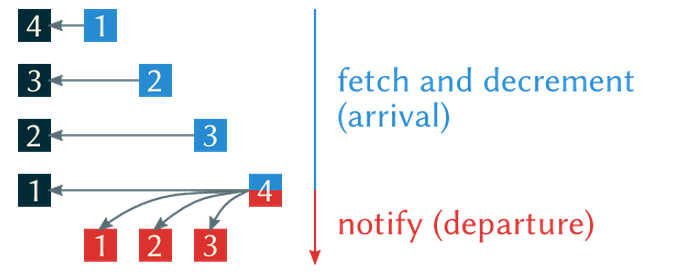
\includegraphics[width=0.5\columnwidth]{central.png}
\end{center}

We chose for this implementation the Sense-Reversing Barrier described by following pseudo
code:
\\
\begin{lstlisting}{c}
(shared) int count = P;
(shared) bool sense = true;
(local) bool local_sense = true;
void central_barrier ()
{
  local_sense = !local_sense;
if(fetch_and_decrement ( &count ) == 1)
  count = P;
  sense = local_sense;
else
  while ( sense != local_sense ); //spin wait
}
\end{lstlisting}
Basically there exists one shared counter initially containing the number of threads. 
Once a thread arrives at the barrier it is atomically decremented and the thread waits
for a global release flag to change state. If the counter’s value reaches zero this flag
is updated to release all waiting threads.
\\\\
Then, we should implement a barrier that is optimized using tournament, dissemination and 
tree structure, step by step.
\\
Following pseudo code describes the function of our tournament barrier implementation:
\begin{lstlisting}{c}
// Shared data:
struct round_t
{
  boolean *opponent
  int role // WINNER or LOSER
  boolean flag
}
round_t rounds[P][logP]
// Private data for each thread:
boolean sense
int parity
round_t *myrounds
procedure tour_barrier
  round_t round=current_v_thread->myrounds;
  for(;;) {
    if(round->role & LOSER) {
      round->opponent->flag = sense;
      while (root_sense != sense);
      break;
    }
    else if (round->role & WINNER)
      while (round->flag != sense);
    else if (round->role & ROOT) {
      while (round->flag != sense);
      champion_sense = sense;
      break;
    }
round++;
}
\end{lstlisting}
Two threads play against each other in each round. The loser thread sets the flag on
which the the winner is busy waiting. Then the loser thread waits for the global
champion flag to be set, where as the winners, play against each other in next
round. The overall winner becomes the champion and notifies all losers about
the end of barrier.
\\\\
Next, we developed a barrier optimized using dissemination.
\begin{center}
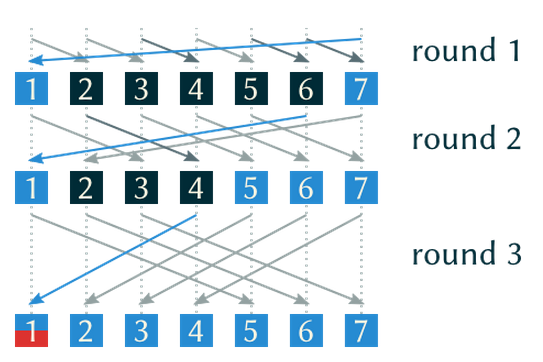
\includegraphics[width=0.5\columnwidth]{diss.png}
\end{center}
Each thread spins
around a variable dedicated to it, and signaled by another thread. Each thread
goes through log(N) rounds where N is the number of threads. At the end of
rounds, the thread knows that the other threads in the system have reached the
barrier and it is good to proceed to the next barrier episode.
\begin{lstlisting}{c}
procedure dissem_barrier {
  i = thread_id;
  sense = thread_private->sense
  parity = thread_private->parity
  for ( r = 0; r < logP; r++) {
    nodes[i][r].partner.flag[parity]= sense;
    while (nodes[i][r].flag[parity] != sense)
  }
  if(parity==1)
    thread_private->sense = sense^1;
  thread_private->parity=1-parity;
}
\end{lstlisting}
Finnaly, we also implemented a barrier optimized by a tree structure.
\begin{center}
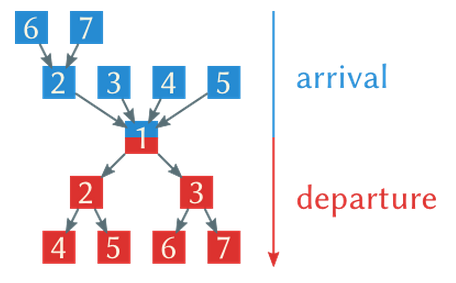
\includegraphics[width=0.5\columnwidth]{tree.png}
\end{center}
In this method, each thread is assigned to a unique tree node which is linked
into an arrival tree by a parent link and into the wakeup tree by a set of child
links. The parent notifies each of its children by setting a flag in the nodes
corresponding to them. The child in turn sets a flag in the parent node to
signal its arrival at the barrier.
\begin{lstlisting}{c}
// Shared data:
typedef struct {
  volatile boolean *parentflag;
  boolean *child_notify[2];
  volatile long havechild;
  volatile long childnotready;
  boolean wakeup_sense;
} treenode;
treenode shared_array[P];
Private data for each thread:
volatile int parity;
volatile boolean sense;
treenode *mynode;
procedure tree_barrier
  vpid=thread_id;
  treenode *mynode_reg;
  mynode_reg = cur_thread->mynode;
  while (mynode_reg->childnotready);
  mynode_reg->childnotready = mynode_reg->havechild;
  *mynode_reg->parentflag = False;
  if (vpid)
    while(mynode_reg->wakeup_sense != cur_thread->sense);
  *mynode_reg->child_notify[0] = cur_thread->sense;
  *mynode_reg->child_notify[1] = cur_thread->sense;
  cur_thread->sense ^= True;
}
\end{lstlisting}

Our performance analysis expose following results for the average barrier latency (in us)
dependent on thread count:
\\
\begin{tabular}{|c|c|c|c|c|c|c|}\hline
   Thread Count & PThread [us] & Counter [us] & Tournament [us] & Dissemination [us] & Tree [us] \\ \hline
   1 & 6.4 & 0.6 & 0.3 & 0.4 & 0.4 \\ \hline
   2 & 726.1 & 4.9 & 7.3 & 3.8 & 3.8  \\ \hline
   4 & 1270.7 & 13.7 & 15.2 & 11.4 & 9.6   \\ \hline
   8 & 2549.8 & 26.8 & 21.8 & 15.7 & 15.0  \\ \hline
   12 & 4712.4 & 53.9 & 32.7 & 23.3 & 21.5  \\ \hline
   16 & 6661.1 & 55.2 & 29.7 & 23.0 & 22.9 \\ \hline
   24 & 10120.6 & 82.5 & 32.8 & 29.1 & 28.3   \\ \hline
   32 & 13769.2 & 114.9 & 40.3 & 33.3 & 32.5 \\ \hline
   40 & 18057.8 & 168.6 & 48.3 & 41.6 & 42.0   \\ \hline
   48 & 20630.7 & 256.0 & 57.1 & 66.3 & 74.4 \\ \hline
\end{tabular}
\\\\
The plot shows that the PThread barrier latency is by far the worst implementation. It 
has a very high latency for a small thread count and is not scaleble at all. Surprisingly,
the simple central barrier implementation returns very good results for a thread count 
to 8 but the scalability is limited as well.
\begin{center}
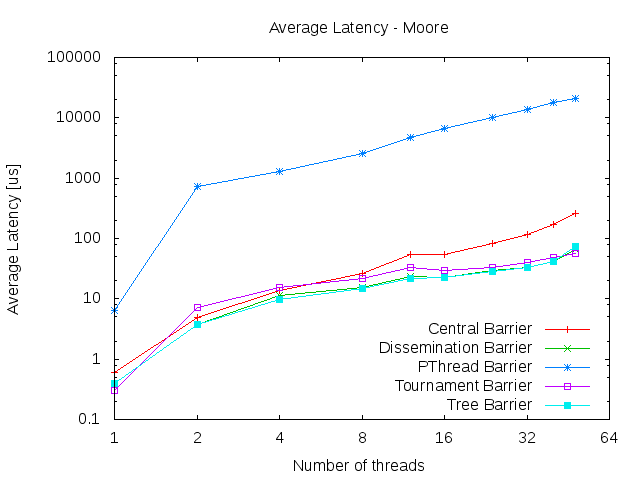
\includegraphics[width=0.8\columnwidth]{ave_latency.png}
\end{center}
The remaining three implementations provide the best and quite equal results, whereas the 
tree barrier has the lowest latency and the tournament barrier has the highest latency.
Yet, all three implementation show a good scalability.
\end{homeworkProblem}

\clearpage
\end{document}
